% This must be in the first 5 lines to tell arXiv to use pdfLaTeX, which is strongly recommended.
\pdfoutput=1
% In particular, the hyperref package requires pdfLaTeX in order to break URLs across lines.

\documentclass[11pt]{article}

% Remove the "review" option to generate the final version.
%\usepackage[review,nohyperref]{acl}
\usepackage{acl}

% Standard package includes
\usepackage{times}
\usepackage{latexsym}

% For proper rendering and hyphenation of words containing Latin characters (including in bib files)
\usepackage[T1]{fontenc}
% For Vietnamese characters
% \usepackage[T5]{fontenc}
% See https://www.latex-project.org/help/documentation/encguide.pdf for other character sets

% This assumes your files are encoded as UTF8
\usepackage[utf8]{inputenc}

% This is not strictly necessary, and may be commented out,
% but it will improve the layout of the manuscript,
% and will typically save some space.
\usepackage{microtype}

% If the title and author information does not fit in the area allocated, uncomment the following
%
%\setlength\titlebox{<dim>}
%
% and set <dim> to something 5cm or larger.

%algo packages
\usepackage{algorithm}
\usepackage{algorithmic}

%color packages
\usepackage{xcolor}
\colorlet{shadecolor}{orange!15}
\usepackage{color,soul}
\usepackage{soulutf8}
\definecolor{bordeau}{rgb}{0.3515625,0,0.234375}

% position of figure
\usepackage[absolute,overlay]{textpos}

%graphic packages
\usepackage[export]{adjustbox}
\usepackage{graphicx}
\graphicspath{ {figures/} }
\usepackage{wrapfig}
\usepackage{float} 
\usepackage{tikz}
\usepackage{pgfplots}
\usepackage{pgfplotstable}

% table packages
\usepackage{array}
\usepackage{multirow,booktabs}
\usepackage{multicol}
\usepackage{tabularx}

% font package
\usepackage[utf8]{inputenc}	% Para caracteres en español
\usepackage{textcomp}
%\usepackage{times}
%\usepackage{lmodern}
\usepackage{mathptmx}

% equation packages
\usepackage{amsmath,amsthm,amsfonts,amssymb,amscd}
\usepackage{mathrsfs}

\usepackage{enumitem}
\setlist{nosep}
\usepackage{latexsym}
\usepackage{graphicx}
\usepackage{xcolor}
\usepackage{longtable}
\usepackage{tikz}
\usetikzlibrary{calc}
\usepackage[draft]{todo}
\usepackage[normalem]{ulem}
\usepackage{xspace}
\usepackage{amsmath,amsfonts,amssymb}

\newcommand{\fyTodo}[1]{\Todo[FY:]{\textcolor{orange}{#1}}}
\newcommand{\fyTodostar}[1]{\Todo*[FY:]{\textcolor{orange}{#1}}}
\newcommand{\fyDone}[1]{\done[FY]\Todo[FY:]{\textcolor{orange}{#1}}}
\newcommand{\fyFuture}[1]{\done[FY]\Todo[FY:]{\textcolor{red}{#1}}}
\newcommand{\fyDonestar}[1]{\done[FY]\Todo[FY:]{\textcolor{orange}{#1}}}
\newcommand{\jcTodo}[1]{\Todo[JC:]{\textcolor{red}{#1}}}
\newcommand{\jcDone}[1]{\done[JC]\Todo[JC:]{\textcolor{red}{#1}}}
\newcommand{\revision}[1]{\textcolor{black}{#1}}
\newcommand{\revisiondone}[1]{\textcolor{black}{#1}}
\newcommand{\revisiondel}[1]{}
\newcommand{\src}{\ensuremath{\mathbf{f}}} % source sentence
\newcommand{\trg}{\ensuremath{\mathbf{e}}} % target sentence
\newcommand{\domain}[1]{\texttt{\textsc{#1}}}
\newcommand{\system}[1]{\texttt{{#1}}}
\newcommand{\SB}[1]{\textbf{#1}}
\newcommand{\SW}[1]{\underline{#1}}
\newcommand{\mtsquare}[0]{MT$^2$}
\newcommand{\lagd}[0]{LaGD$^2$}

\makeatletter
\newenvironment{breakablealgorithm}
  {% \begin{breakablealgorithm}
   \begin{center}
     \refstepcounter{algorithm}% New algorithm
     \hrule height.8pt depth0pt \kern2pt% \@fs@pre for \@fs@ruled
     \renewcommand{\caption}[2][\relax]{% Make a new \caption
       {\raggedright\textbf{\fname@algorithm~\thealgorithm} ##2\par}%
       \ifx\relax##1\relax % #1 is \relax
         \addcontentsline{loa}{algorithm}{\protect\numberline{\thealgorithm}##2}%
       \else % #1 is not \relax
         \addcontentsline{loa}{algorithm}{\protect\numberline{\thealgorithm}##1}%
       \fi
       \kern2pt\hrule\kern2pt
     }
  }{% \end{breakablealgorithm}
     \kern2pt\hrule\relax% \@fs@post for \@fs@ruled
   \end{center}
  }
\makeatother

%subfigure
\usepackage{caption}
\usepackage{subcaption}

%\title{Multi-domain, multilingual translation with latent multi-task group dropout}
\title{Latent Group Dropout for Multilingual and Multidomain Machine Translation}
% Author information can be set in various styles:
% For several authors from the same institution:
% \author{Author 1 \and ... \and Author n \\
%         Address line \\ ... \\ Address line}
% if the names do not fit well on one line use
%         Author 1 \\ {\bf Author 2} \\ ... \\ {\bf Author n} \\
% For authors from different institutions:
% \author{Author 1 \\ Address line \\  ... \\ Address line
%         \And  ... \And
%         Author n \\ Address line \\ ... \\ Address line}
% To start a seperate ``row'' of authors use \AND, as in
% \author{Author 1 \\ Address line \\  ... \\ Address line
%         \AND
%         Author 2 \\ Address line \\ ... \\ Address line \And
%         Author 3 \\ Address line \\ ... \\ Address line}

\author{MinhQuang Pham$^{\dag\ddag}$\thanks{$\ \ \ \ $Now Research Scientist at Zoom Video Communications}, \ \ Josep Crego$^\dag$,\ \ Fran\c cois Yvon$^\ddag$ \\
  $^\dag$SYSTRAN / 5 rue Feydeau, 75002 Paris, France\\
  {\tt firstname.lastname@systrangroup.com}\\
  $^\ddag$Universit\'e Paris-Saclay, CNRS, LIMSI,  91405 Orsay, France\\
  {\tt firstname.lastname@limsi.fr}} 


\begin{document}
\setlength{\abovedisplayskip}{3pt}
\setlength{\belowdisplayskip}{3pt}
\maketitle

\begin{abstract}
  Multidomain and multilingual machine translation often rely on parameter sharing strategies, where large portions of the network are meant to capture the commonalities of the tasks at hand, while smaller parts are reserved to model the peculiarities of a language or a domain. In adapter-based approaches, these strategies are hardcoded in the network architecture, independent of the similarities between tasks. In this work, we propose a new method to better take advantage of these similarities, using a latent-variable model. We also develop new techniques to train this model end-to-end and report experimental results showing that the learned patterns are both meaningful and yield improved translation performance without any increase of the model size. 
\end{abstract}

\section{Introduction}
Multidomain and multilingual machine translation aim to develop one single model to perform translation for multiple domains and multiple language pairs, respectively.\footnote{We will refer to these two situations as 'multi-task MT' and refer to individual domains and languages as 'tasks'.} These paradigms are motivated by the compactness of the resulting translation system \citep{Chu18multilingual,dabre20survey}, the hypothetical positive knowledge transfer between similar domains \citep{Pham21revisiting} or between languages in the same family \citep{Tan19multilingual}. However, having all the tasks use exactly the same model parameters can cause negative interference between unrelated tasks \citep{conneau20unsupervised,wang20negative}. Hence, the recent development of approaches relying on a partial sharing of the parameters, eg.\ using adapter layers as studied in \citep{houlsby19parameter,Bapna19simple,Pham20Study,Philip20monolingual}. If these techniques have proven effective for building strong baselines, they fail to fully take advantage of the similarities that exist between domains and tasks, as documented eg.\ in \citep{Pham21revisiting}. This is because the partition of the parameter space between generic or task-specific subparts, and their allocation to each task, is hard-coded in the network, irrespective of the actual commonalties and differences in the data space.

In this work, we study and develop a new method, \emph{multi-task group dropout}, aimed to take into account the similarity between tasks in a more effective way, by \emph{learning the network organization from the data}. To this end, we introduce a set of latent variables in the model, to account for the unseen association between tasks and regions of the representation space and show how training can still be performed end-to-end using a variational surrogate of the log-likelihood loss function. Our experiments with multilingual and multidomain machine translation confirm that this method can automatically detect similarities in the data, meaning that related tasks use the same subparts of the network. Our results also show that this method is comparable to using adapter layers in a number of empirical comparisons; however, contrarily to adapters, these performance are obtained without any increase of the model size. Our contributions are primarily methodological and can be summarized as follows:
\begin{enumerate}
  \setlength{\itemsep}{1pt}
  \setlength{\parskip}{0pt}
  \setlength{\parsep}{0pt}
\item We introduce a novel, sound mathematical formulation to the problem of jointly learning task-dependent sub-networks and the parameters of the underlying models using variational probabilistic modeling techniques;
\item We present algorithms to train this model end-to-end with very little extra parameters;
\item We report, using an extensive set of experiments, gains for multidomain MT and very low-resourced languages in multilingual MT;
\item We study how this method can actually exploit the similarities between tasks to learn interpretable sub-networks.
\end{enumerate}
\fyDone{Can you do distillation ? That is only keep the parameter for one domain and still get good results (better than DA ?)}

\section{Multi-task group dropout \label{sec:architecture}}
\subsection{Network architecture, groups and layers}
Many architectures for multitask learning are based on a matching of subset of model parameters with tasks. Given the task and the input instance, only a subpart of the network will be involved in the computation of the output value, based on a predefined association between subnetworks and tasks. The adapter architecture of \citep{Bapna19simple} illustrates this strategy, where a task-dependent set of layers is activated for each task. 

In our approach, we also require to know the task $d \in [0 \dots n_d-1]$ for each training and test instance. The structure of our Transformer networks \citep{Vaswani17attention} is however based on the notion of \emph{groups of nodes in the computation graph}. At the input of each Transformer layer $l \in [1 \dots L]$, we partition all input state vectors into $n_p$ groups of nodes, and zero-out a task-dependent subset of these groups.\fyDone{In the attention heads only? In the FF?} The assignment of tasks to groups will be learned from the data, under the constraint that each task only activates exactly $k$ groups of \emph{active nodes}, while the all the other values are nullified, akin to a dropout process (see Figure~\ref{fig:group_dropout}).
\begin{figure}
  \centering
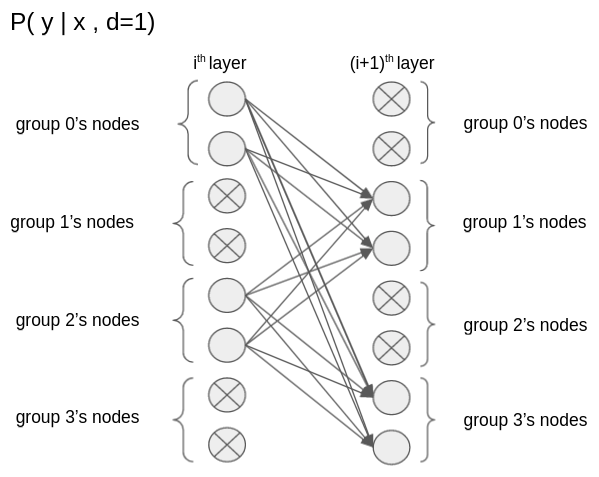
\includegraphics[width=0.4\textwidth]{group_dropout}
\caption{Latent group dropout. The set of nodes\fyDone{parameters ?} in each layer is divided into equal-sized groups. For each task, we only keep a fixed number of active groups of nodes and nullify all the other nodes.
%  Our method learns which groups will be kept / dropped for each task.
}
\label{fig:group_dropout}
\end{figure}
Formally, a \emph{group dropout mask} $m_l^d$ is a $n_p$-dimensional binary vector containing exactly $k$ ones: group $p$ ($\in  [0,\dots,n_p\text{-}1]$) is retained for task $d$ if $m_l^d(p) =1$ and is dropped if $m_l^d(p) = 0$. We denote $\Delta^{n_p}_k = \{ m \in \{0,1\}^{n_p} \text{ such that }  \mid{} m \mid_{L_1} = k \}$ the set of all admissible masks, with $\mid{} m \mid_{L_1}$ the $L_1$ norm of vector $m$; $\#\Delta^{n_p}_k$ is the cardinal of $\Delta^{n_p}$.

Given $m_l^d$, the mask $r_l^d$ for task $d$ in layer $l$ is then derived as:
\begin{align*}
  r_l^d(i) = m_l^d(p) \ \ \ \text{if}\ \ \ p \times \frac{d_k}{n_p} \leqslant i < (p+1) \times \frac{d_k}{n_p},
%  \begin{cases}
%    1, & \text{if}\ p \times \frac{d_k}{n_p} \leqslant i < (p+1) \times \frac{d_k}{n_p} \\
%    & \text{AND} \  m_l^d(p) \text{\small =} 1 \\
%    0, & \text{otherwise},
%  \end{cases} 
  % p & \in  \{0,\dots,n_p\text{-}1 \}, \\
  % d & \in  \{0,\dots,n_d\text{-}1 \}, \\
  % i & \in  \{0,\dots,d_k\text{-}1 \}, \\
  % m_l^d & \in  \{0,1\}^{n_p} \ \forall d,l \, \\
  % \mid m_l^d \mid_{L_1} & =  k , \\
  % \Delta^{n_p}_k & =  \{ m \in \{0,1\}^{n_p} | \mid m \mid_{L_1} = k \},
\end{align*}
where $d_k$ is the dimension of the hidden state.\fyDone{Check this} The propagation of information within the network then depends on the current task value as follows:
\begin{align*}
  \forall l \in [0,\cdots, L-1]: \tilde{h}^l &= h^l \odot r_l^d ,\\
  h^{l+1} &= \operatorname{LAYER}^{l+1}(\tilde{h}^l) ,
\end{align*}
where $\operatorname{LAYER}^l()$ represents all the computations in Transformer layer $l$, $\odot$ is element-wise product. It is applied at all positions of each layer in the encoder and in the decoder.  
% The dropping mask $r_l^d$ is computed as follows
% where $n_p$ is the number of dropout groups; $n_d$ is the number of domains; $d_k$ is the size of Transformer layers; $k$ is the number of retained groups at each layer; $m_l^d$ is a binary vector indicating which group of the nodes of the $l^{th}$ layer is dropped in the sub-network modeling domain $d$. 

\subsection{Training with latent dropout masks}
Assuming standard notation for our translation model  $P(y|x,d;\theta)$ where $x$, $y$ and $\theta$ respectively refer to the input, output, and parameter vector, the latent variables $m_{l}^d, l \in[0,\dots,L], d \in [0, \dots, n_d-1]$ are introduced as follows. We chose the prior distribution for $m_{l}^d$ as the uniform distribution over $\Delta^{n_p}_k$: $P(m_l^d | x, d; \theta) = \operatorname{Unif}(\Delta^{n_p}_k)$; variables for each layer are independent and collectively refered to as $m^d$. For any (variational) distribution $Q(m^1 \dots m^{n_d}; \Phi)$ with parameters $\Phi=\{\phi_l^1, ..., \phi_L^{n_d}\}$, it is well-known that the log-likelihood is lower-bounded by the so-called $\operatorname{ELBO}$ function (hereafter denoted $\ell$), made of a summation of two terms: the \emph{distortion} $D$ and the \emph{rate} $R$ defined as follows:%\footnote{We drop the dependency in $x$ to avoid notational clutter.}
\begin{align}
  \log P(y|x,d;\theta) \ge & \ell(x,y,d; \theta, \Phi) \nonumber \\
  \ell(x,y,d; \theta, \Phi) =&  D(x,y,d; \theta, \Phi) - R(x,y,d; \theta, \Phi) \label{eq:lower-bound}\\
  D(x,y,d; \theta, \phi) = & \mathbb{E}_{m^d \sim Q(m^d |d,\Phi)} \log P(y | m^d, x, d; \theta) \nonumber\\
  R(x,y,d; \theta, \phi) = & \operatorname{KL}(Q(m^d | d, \Phi)||P(m^d | x,d; \theta)), \nonumber
\end{align}
where $\operatorname{KL}$ is the Kullback-Leibler divergence. We use $-\ell(x,y,d; \theta,\Phi)$ as our surrogate training loss, as a tractable approximation of the likelihood, and try to minimize this function in $\theta$ and $\Phi$.

The variational distribution $Q$ of $m^d$ is defined independently on a layerwise basis; this means that each layer only involves a subset $\Phi_l^d$ of variational parameters. $Q$ is computed as follows:
\begin{align}
  \operatorname{Ind}^d = \{ i_1, \cdots, i_k \} & \sim \text{SRS}(\operatorname{softmax}(\Phi_l^d), k) \nonumber \\
  m_l^d(i) & =  \text{$\mathbb{I}$}(i \in \operatorname{Ind}^d), \nonumber
\end{align}
where $\text{SRS}(\pi,k)$ denotes the process of sampling $k$ times without replacement from the distribution $\pi$, and $\mathbb{I}$ is the indicator function. This modeling choice for the latent vector $m_l^d$ is motivated by the Gumbel Top-K trick of \citet{Kool19stochastic} that we use below.  Given our choices for the prior and the variational distributions, the two terms in Eq.~\eqref{eq:lower-bound} can be computed as:
\begin{align}
\hspace{-2.em}
D(\dots) &= \mathbb{E}_{m^d \sim Q(m^d | d; \Phi)} \text{log} P(y | m^d, x, d, \theta) \nonumber \\
&= \mathbb{E}_{g^d \sim^{\text{i.i.d}} G(0,1)} \big[ \log P(y |\tilde{m}^d, x, d, \theta,) \big] \nonumber
\end{align}
where the generation process $G(0,1)$ is a product of independent Gumbel distributions, yielding:
\begin{align}
  \hspace{-2.em}
  \forall d,  g^d & =  [g_1^d, \dots, g_L^d],  \text{ with } g_l^d \in \mathbb{R}^{n_p} \nonumber \\
  \forall p,  g_l^d(p) & \displaystyle{\mathop{\sim}^{\text{i.i.d}}} \operatorname{Gumbel}(0,1) \nonumber \\
  \operatorname{Ind}^d = \{ i_1, \cdots, i_k \} &= \operatorname{Top-k} \ \{ \ g_l^d(0) + \Phi_l^d(0), \cdots, \nonumber \\ 
       & \quad \quad g_l^d(n_p\text{-}1) + \Phi_l^d(n_p\text{-}1) \ \}\label{eq:top-k} \\
\tilde{m}_l^d(p) &= \mathbb{I}(p \in Ind^d). \nonumber 
\end{align}
For the second term, the derivation is the following:\fyDone{Check this: we have a sum over layers ?Also: R or -R ?} 
\begin{align}
\hspace{-2.em}
  R    &= \operatorname{KL}(Q(m^d | d, \Phi)||P(m^d | x, d; \theta)), \nonumber \\ 
	&= -\sum_{l=1}^L \big(\mathbb{H} \big[ Q(m_l^d | d, \Phi) \big] - \text{log}(\#\Delta^{n_p}_k) \big) \nonumber \\ 
	&= -\sum_{l=1}^L \big(\mathbb{H} \big[ Q(i_1,\cdots,i_k | d, \Phi) \big] - \text{log}(\#\Delta^{n_p}_k) \big)\nonumber \\
	&\leqslant  -\sum_{l=1}^L \big(\mathbb{H} \big[ Q(i_1 | d, \Phi_l^d) \big] - \text{log}(\#\Delta^{n_p}_k) \big). \label{eq:entropy}
\end{align}
We prove inequality~\eqref{eq:entropy} in Appendix~\ref{appendix:b}.
This inequality shows that an upperbound of $R$ is $\sum_{l=1}^L(\text{log}(\#\Delta^{n_p}_k) - \mathbb{H}(\text{softmax}(\Phi_l^d)))$ since $i_1 | \Phi_l^d \sim \operatorname{softmax}(\Phi_l^d)$. During training, we thus maximize a sum over layers of the entropy $\mathbb{H}(\text{softmax}(\Phi_l^d))$\fyDone{Check sum} which performs a regularization over the parameters $\Phi^d$ of the variational distribution. 

Thanks to the Gumbel Top-K trick, we can move the parameters $\Phi$ into the objective function and get rid of policy gradients, which have been reported to be very unstable \citep{Diederick14auto}. However, the operator $\operatorname{Top-k}$, which serves to define $\tilde{m}_l^d$ in Equation~\eqref{eq:top-k}, is not differentiable. Therefore, we approximate this function by the $\operatorname{Soft-Top-K}$ function defined as follows:
\begin{align}\label{eq:soft-top-k}
\hat{m}_l^d(\tau) &= \displaystyle{\mathop{argmin}_{\substack{
                    0 \leqslant m_i \leqslant 1 \\
  \forall 0 \leqslant i \leqslant n_d\text{-}1 \\
        1^{T}.m = k
      }}} -(g_l^d+\Phi_l^d)^{T} . m - \tau H_b(m) 
\end{align}
in which
\begin{align}
H_b(m) &= - \sum_i m_i \text{log}(m_i) + (1-m_i)\text{log}(1-m_i). \nonumber 
\end{align}

In Appendix \ref{appendix:a}, we prove that $\lim_{\tau \rightarrow 0}\hat{m}_l^d(\tau) = \tilde{m}_l^d$. Furthermore, we also provide the computation of $\hat{m}_l^d(\tau)$ and prove that $\hat{m}_l^d(\tau)$ is a differentiable function w.r.t $\Phi_l^d$ and that its gradients can be computed using the implicit differentiation theorem. During training, we approximate $\tilde{m}_l^d$ by $\hat{m}_l^d(\tau)$ by gradually decaying the hyper-parameter $\tau$ to $0.2$. The gradient of $D$ w.r.t $\Phi_l^d$ is computed using the chain rule as follows:
\begin{align*}
\frac{\partial D}{\partial \Phi_l^d} = \frac{\partial D}{\partial \hat{m}_l^d(\tau)} \times \frac{\partial \hat{m}_l^d(\tau)}{\partial \Phi_l^d} 
\end{align*}
The gradient $\frac{\partial D}{\partial \hat{m}_l^d(\tau)}$ is computed via autograd algorithm while $\frac{\partial \hat{m}_l^d(\tau)}{\partial \Phi_l^d}$ is computed via implicit differentiation, as explained in Appendix~\ref{appendix:a}.

We jointly train the Transformer parameters $\theta$ and the parameters of the variational distribution $\Phi$ using the following multi-task loss.\fyDone{This is repeated}
\begin{align*}
\hspace{-0.em}
\mathcal{L}(\theta,\Phi) = \sum_{d=1}^{n_d} \mathbb{E}_{x \sim \mathcal{D}_s^d,y \sim MT^d(x)} \big[-\ell(x,y,d; \theta,\Phi)\big]
\end{align*}

in which $\mathcal{D}_s^d$ is distribution of task $d$ over the input space $\Omega^d_s$; $\operatorname{MT}^d: \Omega^d_s \rightarrow \Omega^d_t$\fyDone{already defined} is the translation function for task $d$, which our multi-task model needs to learn; $-\ell(x,y, d, \theta,\Phi)$ is the $\operatorname{ELBO}$ loss, defined in Equation~\ref{eq:lower-bound}.

Finally, during inference, we define the dropout mask for layer $l$ and task $d$ as follows:
\begin{align*}
  Ind_l^d &= \operatorname{Top-k}(\Phi_l^d) \\
  m_l^d &= \mathbb{I}(i\in Ind_l^d)
\end{align*}
meaning that we simply pick the $k$ most likely parameter groups for the task at hand, and define the state dropout mask accordingly.

\section{Experimental settings \label{sec:experiments}}

\subsection{System design and configuration}
\subsubsection{Multidomain translation systems}
Our systems for the multidomain experiments are designed as follows:
\begin{itemize}
\item Transformer: The embedding dimension for both encoder and decoder is set as 512, and the feedforward dimension is 2048; the multi-head attention mechanism contains 8 heads; 6 layers in the encoder; 6 layers in the decoder.\fyDone{How many layers}
\item Adapter-based Transformer: the intermediate feedforward dimension is set to 2048, as in \citet{Pham21revisiting}.
\item Transformer using Latent multi-task group dropout (\system{LaMGD} Transformers):\fyDone{Explain acronym} There is no change in the architecture. We group the 512 nodes in each layer into 16 groups of 32 consecutive nodes. For each domain, only 12 out of the 16 groups are selected. The number of parameters of the variational distribution is $L\times k \times L \times n_d$, which is negligible in comparison to the size of the Transformer model.
\item Transformer using heuristic multi-task group dropout (\system{HMGD} Transformer): we share 320 nodes for every task, and reserve 32 nodes for each task (totalling $320 + 32*6 = 512$ nodes).
\end{itemize}

We set the dropout probability to 0.1. We train the multidomain Transformer model for 200k iterations with a batch size of 12k tokens using 4 V100 GPUs. The convergence of the standard Transformer is before 200K as its validation curve became flat near the 200K-th iteration. The \system{LaMGD} Transformer converged after 300k iterations with the same batch size. The convergence of \system{LaMGD} is controlled by its validation curve. Finally, we plug adapters to the multidomain Transformer model and finetune them for 25k iterations using the same batch size as the baseline.
%: this ensures that \system{LaMGD} and Adapter-based Transformer have the same amount of training iterations.

\subsubsection{Multilingual translation systems}
The systems used in our multilingual experiments are implemented as follows:
\begin{itemize}
\item Multilingual Transformer: the embedding dimension for both encoder and decoder is set as 512, and the feedforward dimension is 1024, each multi-head attentions contains 8~heads as in \citep{Wang20balancing}.
\item Adapter based Transformer: the intermediate feedforward dimension is set as 128. We follow here the parameter setting of \citep{Gong21adaptive}.
\item \system{LaMGD} Transformer: There is no change in the architecture. We group 512 nodes in each layer into 16 groups of 32 consecutive nodes. For each language, we select 12 groups.
\end{itemize}

We set the dropout probability to 0.3. We train the multilingual Transformer model for 40k iterations with a batch size of 9600 tokens on 16 V100 GPUs as in \citet{Gong21adaptive}. We train \system{LaMGD} Transformer for 50k iterations with the same batch size. The convergence of the models are controlled via their validation curves. Finally, we finetune the language-specific Adapters for 5k iterations.

All the translation systems are implemented with OpenNMT-tf \footnote{\url{https://github.com/OpenNMT/OpenNMT-tf}} \cite{Klein17opennmt}.\fyDone{Fix this, add reference to framework if needed}

\subsubsection{Hyper-parameters}
\label{ssec:hyperparams}
We choose $n_d = 16$ so that the size of the dropout group is neither too small nor too large. The second important hyper-parameter in \system{LaMGD} is the number of selected groups in each layer, $k$, which we set to 12 in every experiments. By retaining $12/16$ groups, we share on average $75 \%$ active groups between two domains or languages. This design ensures that the percentage of sharing is in the same ballpark as what we obtain with adapter modules. In our future work, we intend to analyze how these choices affect the final performance of the model.

The temperature parameter $\tau$ for the $\operatorname{Soft-Top-K}$ operator is gradually decreased from $0.5$ to $0.2$ according to the following policy:
\begin{align*}
\tau = \operatorname{min}\{ 0.2, 0.5 * \exp^{-r*step} \},
\end{align*}
in which $r=0.0001$.
While \citet{Gong21pay,Gong21adaptive} fixed $\tau$ to be 0.2, we select an anneal policy for $\tau$ proposed by previous studies \citep{Jang17categorical}. Finally, we set the weight of the entropy term to $0.0001$ in the training loss in every experiments.
%$\mathbb{H}(\text{softmax}(\Phi_l^d))$
\subsubsection{Latent variables initialization}
We initialize the distribution of the latent variables uniformly. More precisely, we set $\Phi_l^d$, which generates the probability of the masks via the softmax activation function, to $0^{n_d}$.
\subsection{Datasets and metrics}
\subsubsection{Multidomain translation}
We use the same data as in the recent work of \citet{Pham21revisiting} on multidomain translation.\fyDone{Add public to the data link} The datasets \footnote{See \url{https://github.com/qmpham/experiments/tree/main/tacl20}} for the multidomain translation experiments are detailed in Table~\ref{tab:Corpora-chap4}. For each domain, the size of the dev set and the test set is 1~K. 
\begin{table*}[h!]
  \centering
  \begin{tabular}{|l|cccccc|} %*{4}{|r|}}
    \cline{2-7} 
    \multicolumn{1}{c|}{} & \multicolumn{1}{c}{\domain{med}} & \multicolumn{1}{c}{\domain{law}} & \multicolumn{1}{c}{\domain{bank}} & \multicolumn{1}{c}{\domain{it}} & \multicolumn{1}{c}{\domain{talk}} & \multicolumn{1}{c}{\domain{rel}} \\
    \hline 
    \# lines & 2609 (0.68) & 501 (0.13) & 190 (0.05) & 270 (0.07) & 160 (0.04) & 130 (0.03) \\
    \# \revisiondone{tokens}  &  133 / 154  &  17.1 / 19.6 &  6.3 / 7.3 &  3.6 / 4.6 &  3.6 / 4.0 &  3.2 / 3.4 \\
    \# \revisiondone{types}  & 771 / 720 & 52.7 / 63.1 & 92.3 / 94.7 & 75.8 / 91.4 & 61.5 / 73.3 & 22.4 / 10.5 \\
    \# \revisiondone{uniq} & 700 / 640 & 20.2 / 23.7 & 42.9 / 40.1 & 44.7 / 55.7 & 20.7 / 25.6 & 7.1 / 2.1 \\
    \hline
  \end{tabular}
  \caption{Corpora statistics: number of parallel lines ($\times 10^3$) and proportion in the basic domain mixture (which does not include the \domain{news} domain), number of tokens in English and French ($\times 10^6$), number of types in English and French ($\times 10^3$), number of types that only appear in a given domain ($\times 10^3$).}
%\domain{med} is the largest domain, containing almost 70\% of the sentences, while \domain{rel} is the smallest, with only 3\% of the data.
\label{tab:Corpora-chap4}
\end{table*}
\subsubsection{Multilingual translation}
We evaluate our model on both one-to-many (O2M) and many-to-one (M2O)
translation tasks borrowing the multilingual translation datasets from past studies. More precisely, we used: 
\begin{itemize}
\item TED8-Related. Following the setting of \citet{Wang20balancing}, we use a subset of translations from \citet{qi18when} between English and eight \emph{related languages}.
\item TED8-Diverse. The dataset consists of parallel sentences between English and eight \emph{diverse languages} as in \citet{Wang20balancing}.
\end{itemize}

The languages used in the multilingual experiments are as follows (see statistics in Table~\ref{tab:Corpora-multilingual}):
\begin{itemize}
\item \textbf{Diverse set}: bos (Bosnian), Bulgarian (bul), French (fra), ell (Greek),
  hin (Hindi), Korean (kor) mkd (Macedonian), mar (Marathi);
\item \textbf{Related set}: Azerbajiani (aze), Belarusian (bel),
  Czech (ces), Galician (glg), Portuguese (por), Russian (rus), Slovak (slk), Turkish~(tur).
\end{itemize}

\begin{table*}[h]
  \centering
  \begin{tabular}{|cccc||cccc|} 
  \hline
    \multicolumn{4}{|c||}{Related} & \multicolumn{4}{c|}{Diverse} \\
                            \multicolumn{1}{|c}{\domain{lang}} & \multicolumn{1}{c}{\domain{train}} & \multicolumn{1}{c}{\domain{dev}} & \multicolumn{1}{c||}{\domain{test}} & \multicolumn{1}{c}{\domain{lang}} & \multicolumn{1}{c}{\domain{train}} & \multicolumn{1}{c}{\domain{dev}} & \multicolumn{1}{c|}{\domain{test}} \\
    \hline 
    Azerbaijani & 5.94k & 671 & 903 & Bosnian & 5.64k & 474 & 463 \\
    Belarusian & 4.51k & 248 & 664 & Marathi & 9.84k & 767 & 1090\\
    Galician & 10.0k & 682 & 1007 & Hindi & 18.79k & 854 & 1243\\
    Slovak & 61.5k & 2271 & 2445 & Macedonian & 25.33k & 640 & 438 \\
    Turkish & 182k & 4045 & 5029 & Greek & 134k & 3344 & 4433\\
    Russian & 208k & 4814 & 5483 &  Bulgarian & 174k & 4082 & 5060 \\
    Portuguese & 185k & 4035 & 4855 & French & 192k & 4320 & 4866\\
    Czech & 103k & 3462 & 3831 & Korean & 205k & 4441 & 5637 \\
    \hline
  \end{tabular}
  \caption{Data Statistics of TED8 Datasets}
\label{tab:Corpora-multilingual}
\end{table*}

For all experiments, we report the BLEU score of \citet{Papineni02bleu} computed with SacreBleu \citep{Post18call}. Statistical significance is computed with compare-mt\footnote{\url{https://github.com/neulab/compare-mt}} \cite{Neubig19compare-mt}. We report significant differences at the level of $p=0.05$.\fyDone{Check this}

\section{Results and analyses}

\subsection{Multidomain translation}
For these experiments, our main results are in Table~\ref{tab:mdmt}, where we observe that the \system{LaMGD} Transformer achieves a significant improvement (+2.78) over the generic \system{Transformer} system with zero extra parameters. Moreover, \system{LaMGD} Transformer achieves performance that are equivalent on average to that of the \system{Adapter} sytems, which is finetuned and contains approximately 25M additional parameters per domain. Variational mask learned from data by \system{LaMGD} also outperforms heuristic dropout mask \system{HMGD} by 0.5 in average.
\begin{table*}[h!]
  \centering
  \begin{tabular}{|p{4cm}|*{7}{r|}} \hline
    Model / Domain & \multicolumn{1}{c|}{\domain{ med}} & \multicolumn{1}{c|}{\domain{ law}} & \multicolumn{1}{c|}{\domain{bank}} & \multicolumn{1}{c|}{\domain{talk}} & \multicolumn{1}{c|}{\domain{ it }} & \multicolumn{1}{c|}{\domain{ rel}} & \multicolumn{1}{c|}{\domain{avg}} \\ \hline 
    \system{Transformer}  \hfill{\footnotesize[65m]} & 40.3 & 59.5 & 49.8 & 36.4 & 49.0 & 80.0  & 52.5\\
    \system{HMGD} Transformer   \hfill{\footnotesize[+0m]}  & \SB{40.4} & 60.4 & 51.9 & 38.7 &	50.8 &	86.80 & 54.8 \\ 
    \revision{\system{Adapter}}   \hfill{\footnotesize[+151m]}  & 39.5 & \SB{61.0} & \SB{53.1} & 37.5 & 49.6 & \SB{91.0} & \SB{55.3} \\ 
    \system{LaMGD} Transformer   \hfill{\footnotesize[+0m]}  & 40.3 & 60.4 & 52.4 & \SB{39.0} & \SB{52.4} & 87.5 & \SB{55.3} \\ 
    \hline
  \end{tabular}
  \caption{Multi-domain translation. Boldface identifies best system for each domain.}
  \label{tab:mdmt}
\end{table*}

\subsubsection{Fuzzy domain separation}
\label{ssec:fuzzy}
For this experiment, we reuse proposal of \citet{Pham21revisiting}, who measure the efficiency of a multidomain NMT system exploiting the proximity between domains. It uses the same data as in the previous experiment; however, the domain \domain{law} is now randomly split into two pseudo-domains \domain{law$_1$} and \domain{law$_2$} of equal size. A truly multidomain system should be able to automatically detect the proximity between \domain{law$_1$} and \domain{law$_2$}, and there should be no significant difference between the performance of a system trained with the six original domains (including \domain{law}) or with the seven domains (including \domain{law} by \domain{law$_1$} and \domain{law$_2$}). \citet{Pham21revisiting} reported a large gap between the two settings when using residual adapters. We replicated this setting and report the results obtained with the \system{LaMGD} Transformer system in Table~\ref{tab:fuzzy}. 

\begin{table*}[h!]
  \centering
  \begin{tabular}{|p{4cm}|*{3}{r|}} \hline
    Model / Domain & \multicolumn{1}{c|}{\domain{law}} & \multicolumn{1}{c|}{\domain{law$_1$}} & \multicolumn{1}{c|}{\domain{law$_2$}} \\ \hline 
    \system{Adapter}   \hfill{\footnotesize[+151m]}  & 61.0 & 60.4 (-0.6) &  60.2 (-0.8) \\ 
    \system{LaMGD} Transformer   \hfill{\footnotesize[+0m]}  & 60.4 & 60.4 (=) & 60.4 (=) \\ 
    \hline
  \end{tabular}
  \caption{Experiments with two similar pseudo-domains}
  \label{tab:fuzzy}
\end{table*}

The results in Table~\ref{tab:fuzzy} show a performance decrease for the adapter-based system when training with two pseudo-domains \domain{law$_1$} and \domain{law$_2$}. In contrast, the \system{LaMGD} model obtains very stable results. In Section~\ref{ssec:abalation}, we show that our algorithm in fact computes the same sub-network for \domain{law$_1$} and \domain{law$_2$}, that allows a full sharing of information between these two pseudo-domains.

\subsection{Multilingual translation}
Results for the multilingual experiments are in Table~\ref{tab:multilingual}.  The \system{LaMGD} Transformer achieves an improvement of 0.42, 0.33, 0.32 in average over the multilingual \system{Transformer} in the O2M-related, M2O-related, M2O-diverse conditions, respectively. Significant gains are observed for languages \domain{bel}, \domain{glg} (both direction), \domain{hin} and \domain{bos} (O2M direction) which are very low-resource languages in our sets. However, \system{LaMGD} Transformer is outperformed by the multilingual \system{Transformer} and language Adapters for the O2M-diverse condition.
\begin{table*}[h!]
  \centering
  \begin{tabular}{|p{4cm}|*{9}{r|}} \hline
    O2M-related & \multicolumn{1}{c|}{\domain{aze}} & \multicolumn{1}{c|}{\domain{bel}} & \multicolumn{1}{c|}{\domain{ces}} & \multicolumn{1}{c|}{\domain{glg}} & \multicolumn{1}{c|}{\domain{por}} & \multicolumn{1}{c|}{\domain{rus}} & \multicolumn{1}{c|}{\domain{slk}} & \multicolumn{1}{c|}{\domain{tur}} & \multicolumn{1}{c|}{\domain{avg}} \\ \hline 
    \system{Transformer}  \hfill{\footnotesize[91.6m]} & 4.8 &7.3&20.8&21.1&39.7&19.8&22.6&15.2&18.9 \\
    \revision{\system{Adapter}}   \hfill{\footnotesize[+13m]} &4.3&6.8&21.1&22&39.7&20&23&15.2&19 \\ 
    \system{LaMGD} Transformer  \hfill{\footnotesize[+0m]}  & 5.2&\SB{9.4}&20.6&\SB{22.8}&39.6&19.6&22.4&15.0&19.3 \\ 
	\hline
    \hline
    M2O-related & \multicolumn{1}{c|}{\domain{aze}} & \multicolumn{1}{c|}{\domain{ bel}} & \multicolumn{1}{c|}{\domain{ces}} & \multicolumn{1}{c|}{\domain{glg}} & \multicolumn{1}{c|}{\domain{por}} & \multicolumn{1}{c|}{\domain{rus}} & \multicolumn{1}{c|}{\domain{slk}} & \multicolumn{1}{c|}{\domain{tur}} & \multicolumn{1}{c|}{\domain{avg}} \\ \hline 
    \system{Transformer}  \hfill{\footnotesize[67.8m]} &11.4&16.6&28.5&	27.1&43.7&24.6&30.3&25.6&26.0 \\
    \revision{\system{Adapter}}   \hfill{\footnotesize[+13m]} &10.1&15.8&28.4&26.8&43.7&24.5&30.2&25.6&25.6\\ 
    \system{LaMGD} Transformer   \hfill{\footnotesize[+0m]}  &11.3&\SB{17.4}&28.6&\SB{28.7}&43.7&24.5&30.7&25.6&26.3 \\ 
    \hline
    \hline
    O2M-diverse & \multicolumn{1}{c|}{\domain{bos}} & \multicolumn{1}{c|}{\domain{mar}} & \multicolumn{1}{c|}{\domain{hin}} & \multicolumn{1}{c|}{\domain{mkd}} & \multicolumn{1}{c|}{\domain{ell}} & \multicolumn{1}{c|}{\domain{bul}} & \multicolumn{1}{c|}{\domain{fra}} & \multicolumn{1}{c|}{\domain{kor}} & \multicolumn{1}{c|}{\domain{avg}} \\ \hline 
    \system{Transformer}  \hfill{\footnotesize[96.9m]} & 10.2&4&12.7&22.2&31.8&34.0&38.3&8.3&20.2 \\
    \revision{\system{Adapter}}   \hfill{\footnotesize[+13m]}  &10.2&4&\SB{13.3}&21.9&32.2&34.1&38.5&8.3&20.3 \\ 
    \system{LaMGD} Transformer   \hfill{\footnotesize[+0m]}&10.1&3.8&12.6&\SB{22.8}&31.8&33.4&38.1&8.1&20.1\\
    \hline 
    \hline
    M2O-diverse & \multicolumn{1}{c|}{\domain{bos}} & \multicolumn{1}{c|}{\domain{mar}} & \multicolumn{1}{c|}{\domain{hin}} & \multicolumn{1}{c|}{\domain{mkd}} & \multicolumn{1}{c|}{\domain{ell}} & \multicolumn{1}{c|}{\domain{bul}} & \multicolumn{1}{c|}{\domain{fra}} & \multicolumn{1}{c|}{\domain{kor}} & \multicolumn{1}{c|}{\domain{avg}} \\ \hline 
    \system{Transformer}  \hfill{\footnotesize[70.4m]} &22.4&9.7&20.5&31.8&37.5&38.7&39.8&19.0&27.4 \\
    \revision{\system{Adapter}}   \hfill{\footnotesize[+13m]}  &22.5&9.4&20.0&30.6&37.2&38.2&39.3&19.0&27.0\\ 
    \system{LaMGD} Transformer  \hfill{\footnotesize[+0m]} &\SB{23.5}&9.6&\SB{21.5}&32.2&37.7&38.6&40.0&18.9&27.7 \\
    \hline
  \end{tabular}
  \caption{Multilingual Translation experiments. Boldface denotes significant gains over \system{Transformer} ($p=0.05$).\fyDone{What is the bold for ?}}
  \label{tab:multilingual}
\end{table*}

\subsection{Similarity between dropping masks}
\label{ssec:abalation}
This section compares the sub-networks learnt for each domain or language pair by computing the average similarity between the corresponding dropout masks concatenated for all the layers of the underlying model. For the multidomain experiment, we analyze the case of pseud-domain separation reported in Section~\ref{ssec:fuzzy} in Figure ~\ref{fig:md-heatmap}. We see that the sub-networks for \domain{law$_1$} and \domain{law$_2$} are identical, yielding a full sharing between the corresponding training sets. Furthermore, we observe a large distance between \domain{rel} and the other domains, which is expected given that \domain{rel} is quite distinct from the other domains. \domain{rel} only share around $75 \%$ its active groups with other domains, as would be obtained by chance in our setting (see Section~\ref{ssec:hyperparams}). In Figure ~\ref{fig:domain}, we visualize the domains using their dropping masks concatenated and mapped to a 2d space using Principal Component Analysis (PCA).

\begin{figure}[h!]
\begin{subfigure}{0.5\textwidth}
  \centering
  % include first image
  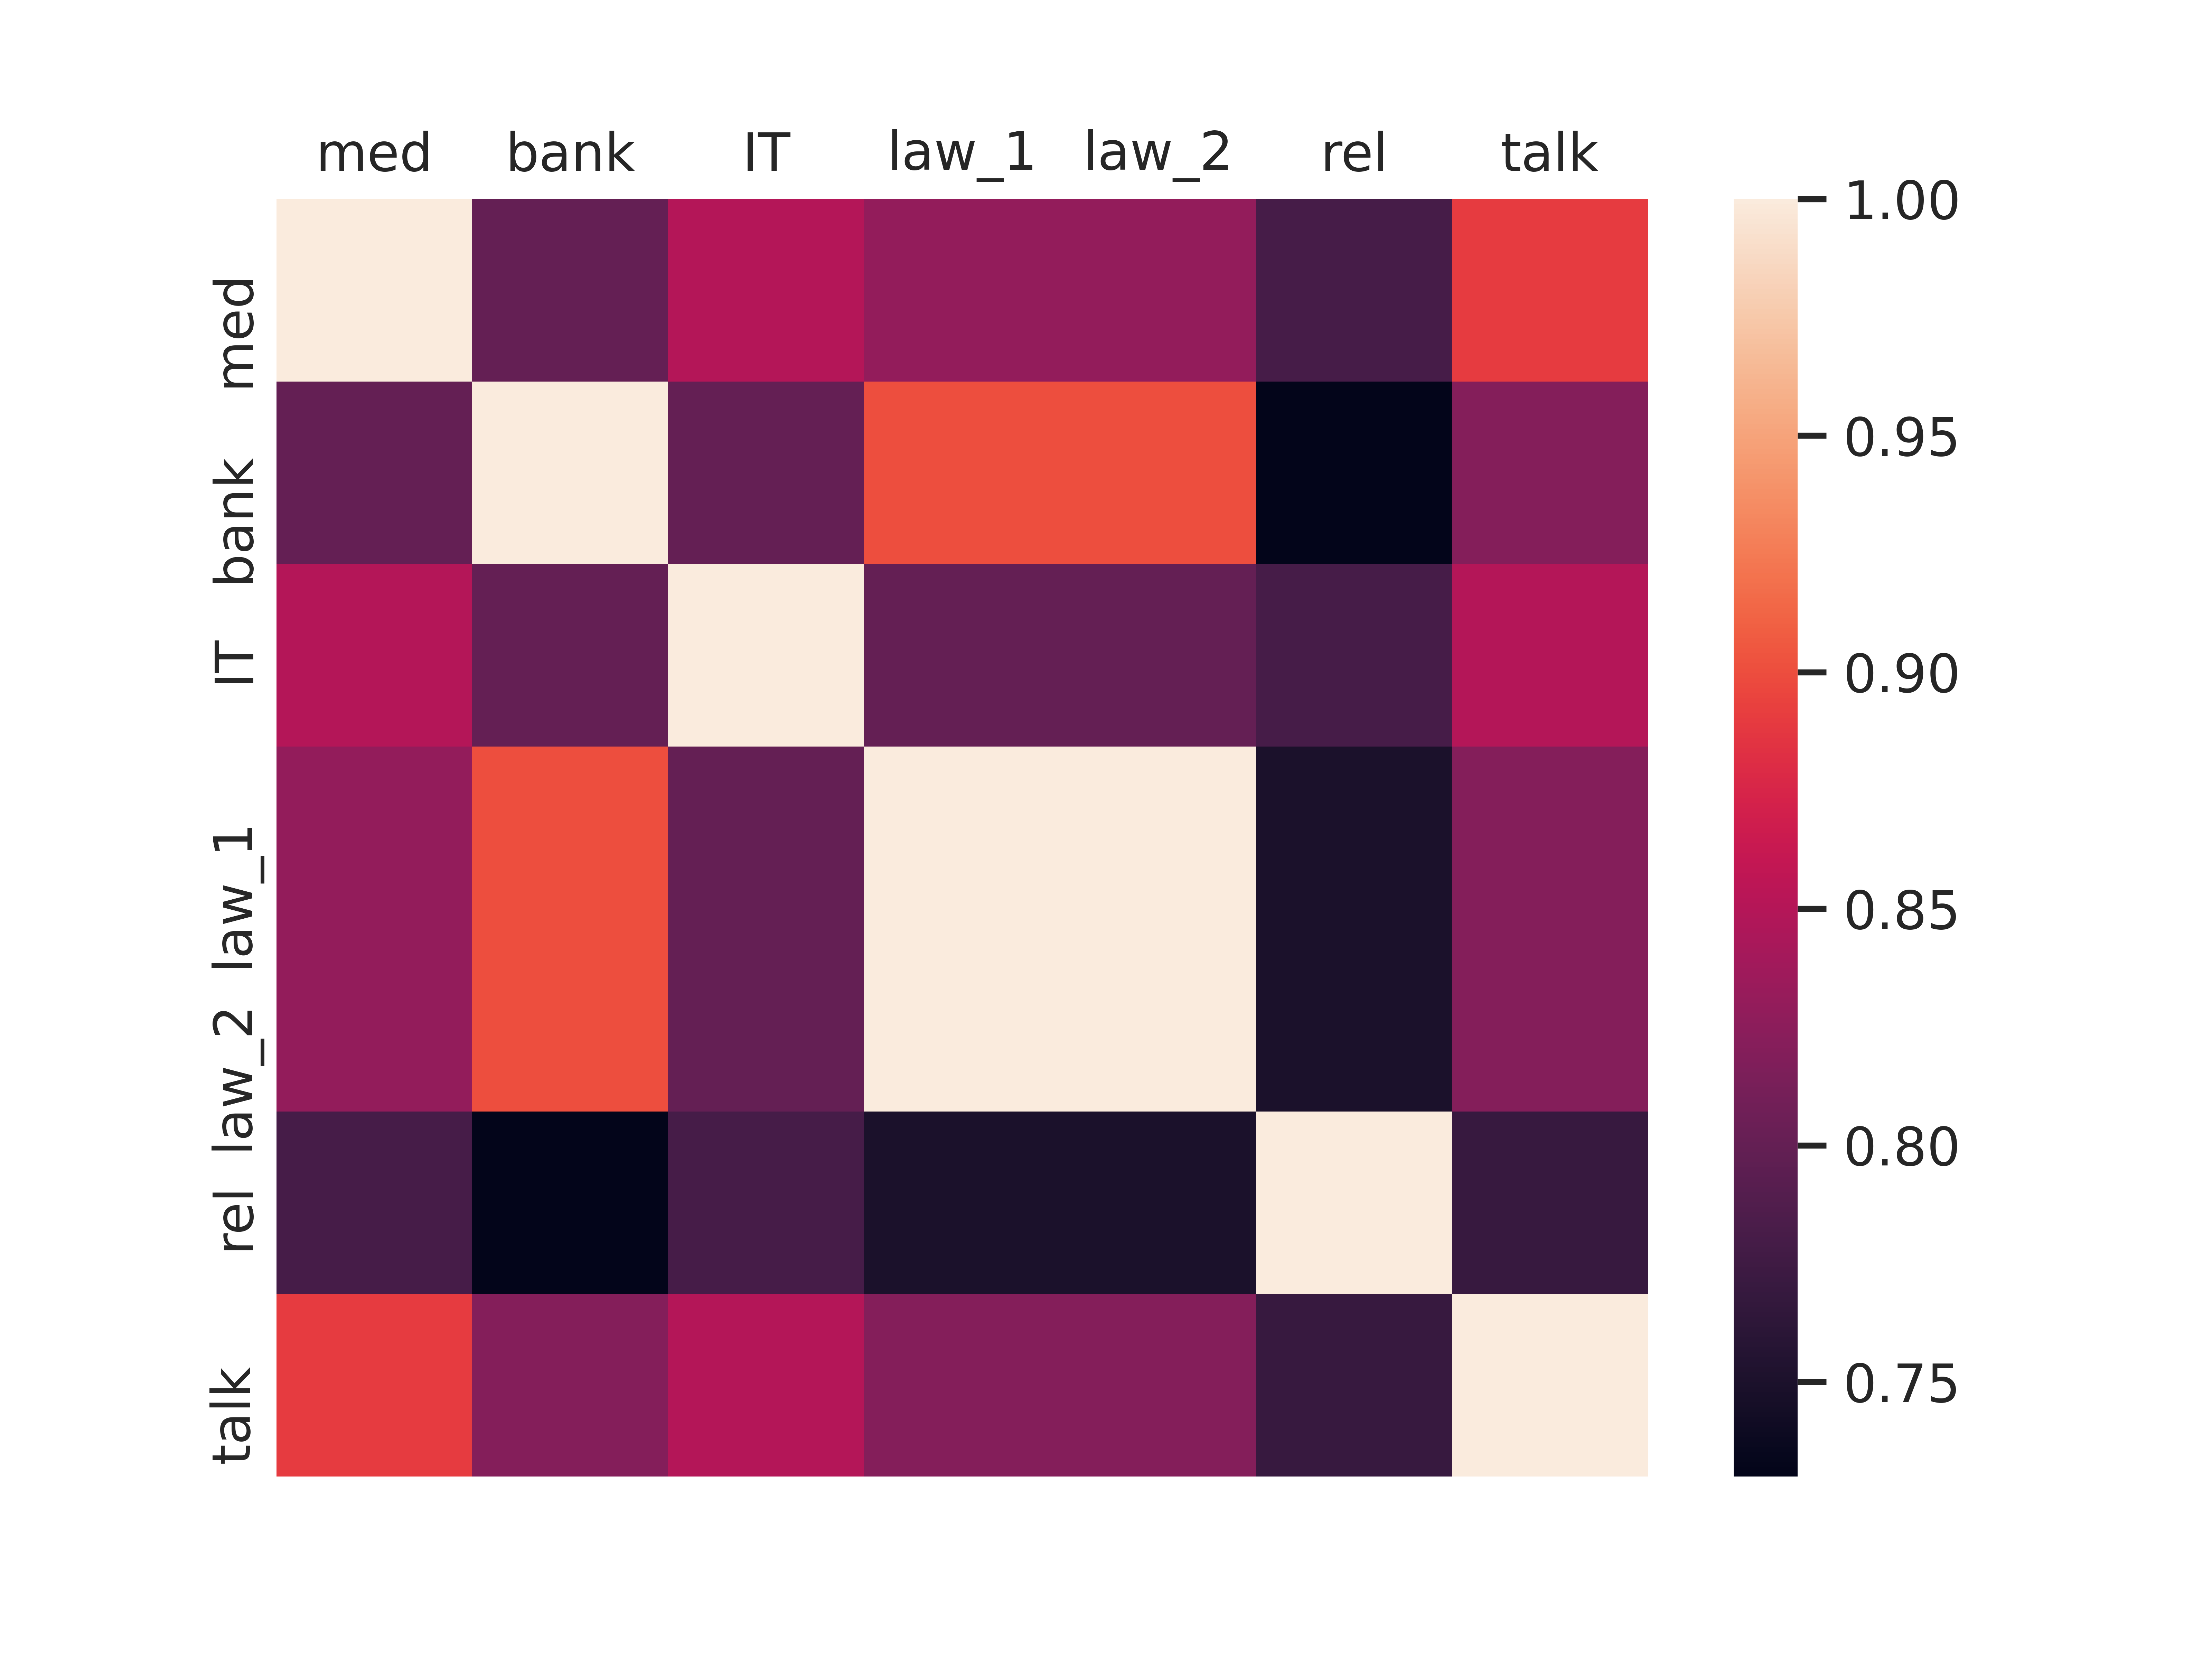
\includegraphics[width=0.7\textwidth]{multi_domain_heatmap.png}  
  \caption{Multidomain}
  \label{fig:md-heatmap}
\end{subfigure}
\begin{subfigure}{0.5\textwidth}
  \centering
  % include second image
  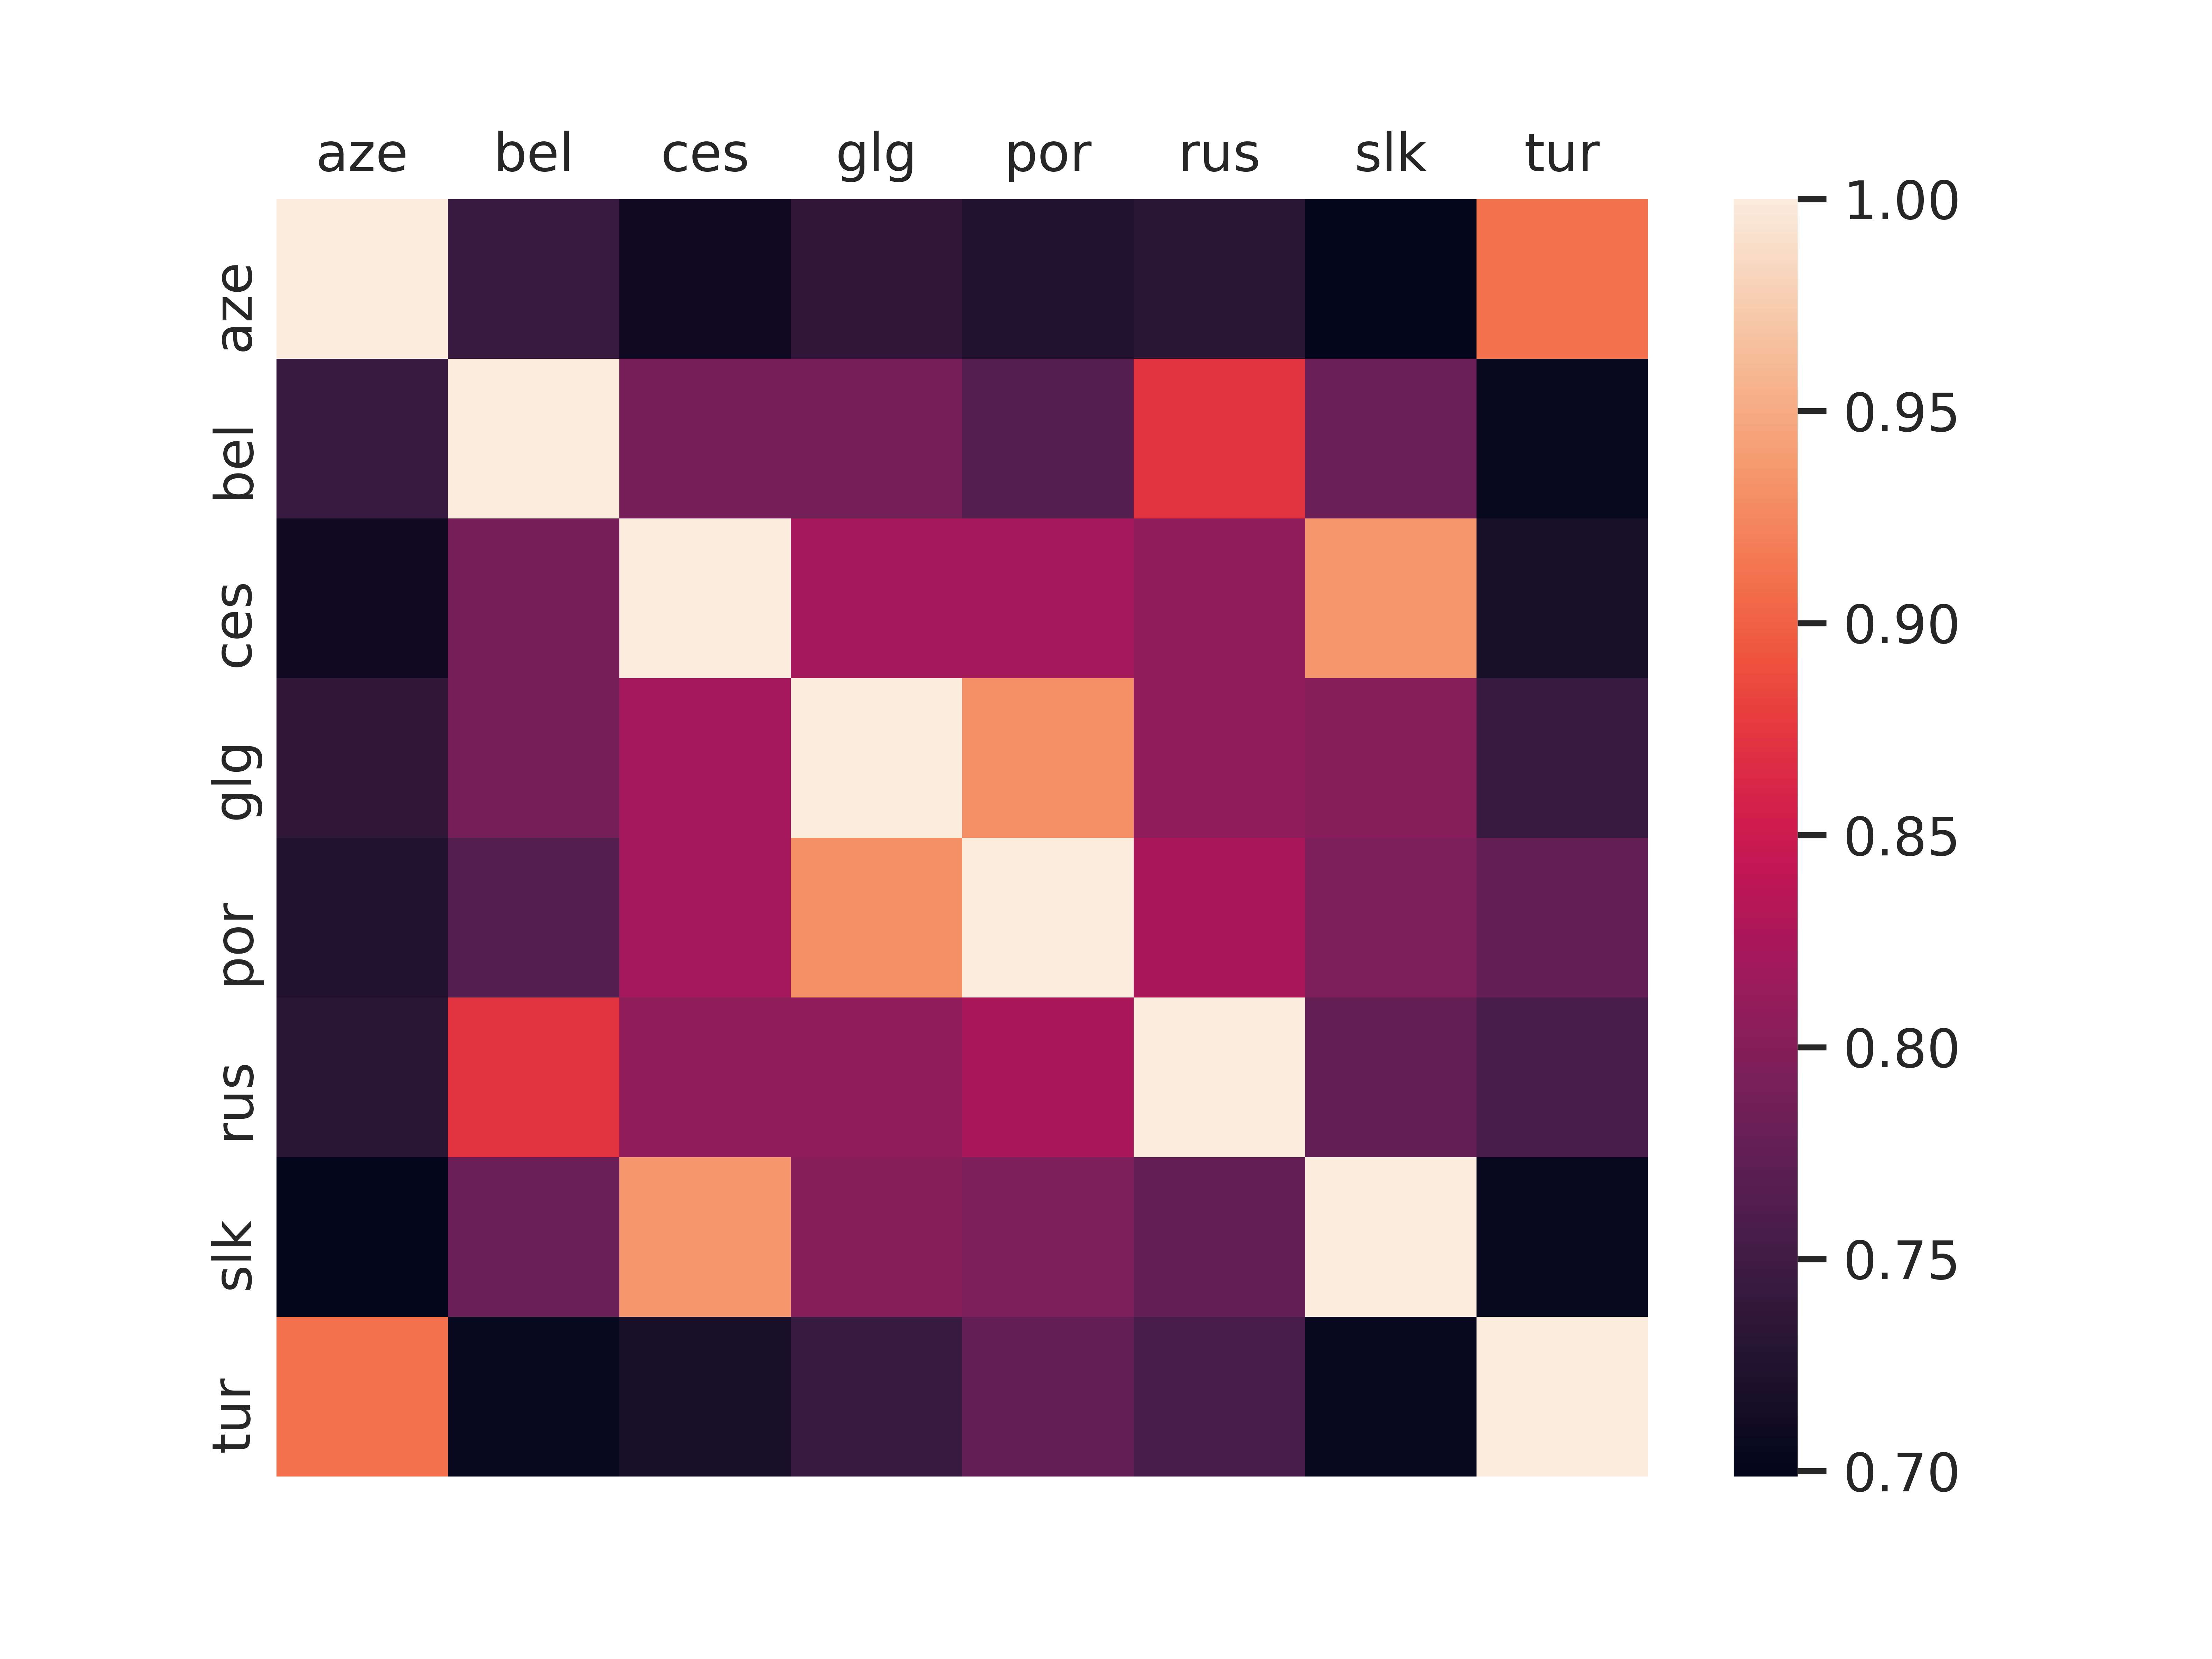
\includegraphics[width=0.7\textwidth]{multilingual_heatmap.png}  
  \caption{Multilingual (Related)}
  \label{fig:ml-heatmap}
\end{subfigure}
\caption{Heatmap visualization of the similarities between dropout masks of domains(languages).}
\label{fig:heatmap}
\end{figure}

%\begin{table*}[h!]
%  \centering
%  \begin{tabular}{|p{1cm}|*{7}{r|}} \hline
%    & \multicolumn{1}{c|}{\domain{ med}} & \multicolumn{1}{c|}{\domain{bank}}& \multicolumn{1}{c|}{\domain{ it }} & \multicolumn{1}{c|}{\domain{law$_1$}} & \multicolumn{1}{c|}{\domain{law$_2$}} & \multicolumn{1}{c|}{\domain{rel}} &\multicolumn{1}{c|}{\domain{talk}} \\ \hline 
%    \domain{med} &1.0&0.80&0.85&0.83&0.83&0.78&0.89\\
%    \domain{bank} &0.80&1.0&0.80&0.90&0.90&0.73&0.82\\
%    \domain{it} &0.85&0.80&1.0&0.80&0.80&0.78&0.85\\
%    \domain{law$_1$} &0.83&0.90&0.80&1.0&\SB{1.0}&0.75&0.82\\ 
%    \domain{law$_2$} &0.83&0.90&0.80&\SB{1.0}&1.0&0.75&0.82\\ 
%    \domain{rel} &0.78&0.73&0.78&0.75&0.75&1.0&0.77\\
%    \domain{talk} &0.89&0.82&0.85&0.82&0.82&0.77&1.0\\
%    \hline
%  \end{tabular}
%  \caption{Multidomain experiments: sub-network similarities}
%  \label{tab:fuzzy-sim}
%\end{table*}      

For multilingual (TED-related) experiments, the training data contains four language families: (1) Turkic, with Azerbaijani and Turkish(\domain{aze},\domain{tur}); (2) Slavic, with Belarusian and Russian (\domain{bel},\domain{rus}); (3) Romance, with Galician and Portuguese (\domain{glg}, \domain{por}); and (4) Czech-Slovak, with Slovak and Czech (\domain{ces}, \domain{slk}). We provide in Figure~\ref{fig:ml-heatmap} the heatmap of the similarities between the dropout masks of our objective languages. We observe that each pair of languages in the same family correspond to brightest color except the diagonal in every column or every row.
%\begin{table*}[h!]
%  \centering
%  \begin{tabular}{|p{1cm}|*{8}{r|}} \hline
%    & \multicolumn{1}{c|}{\domain{aze}} & \multicolumn{1}{c|}{\domain{bel}}& \multicolumn{1}{c|}{\domain{ces}} & \multicolumn{1}{c|}{\domain{glg}} & \multicolumn{1}{c|}{\domain{por}} & \multicolumn{1}{c|}{\domain{rus}} &\multicolumn{1}{c|}{\domain{slk}}&\multicolumn{1}{c|}{\domain{tur}} \\ \hline 
%    \domain{aze} &1.0&0.90&0.89&0.86&0.85&0.91&0.89&\SB{0.95}\\
%    \domain{bel} &0.90&1.0&0.94&0.91&0.91&\SB{0.94}&0.94&0.88\\
%    \domain{ces} &0.89&0.94&1.0&0.92&0.94&0.98&\SB{0.99}&0.91\\
%    \domain{glg} &0.86&0.91&0.92&1.0&\SB{0.96}&0.92&0.93&0.86\\ 
%    \domain{por} &0.85&0.91&0.94&\SB{0.96}&1.0&0.93&0.94&0.87\\ 
%    \domain{rus} &0.91&\SB{0.94}&0.98&0.92&0.93&1.0&0.98&0.93\\
%    \domain{slk} &0.89&0.94&\SB{0.99}&0.93&0.94&0.98&1.0&0.91\\
%    \domain{tur} &\SB{0.95}&0.88&0.91&0.86&0.87&0.93&0.91&1.0\\
%    \hline
%  \end{tabular}
%  \caption{Multilingual sub-networks' similarities (M2O Ted-related). Boldface denotes the similarity of languages in a same family.}
%  \label{tab:related-sim}
%\end{table*}

We also plot the languages based on their dropout masks in Figure~\ref{fig:visual} using a 2d PCA projection.
\begin{figure*}[htbp]
\begin{subfigure}{0.5\textwidth}
  \centering
  % include first image
  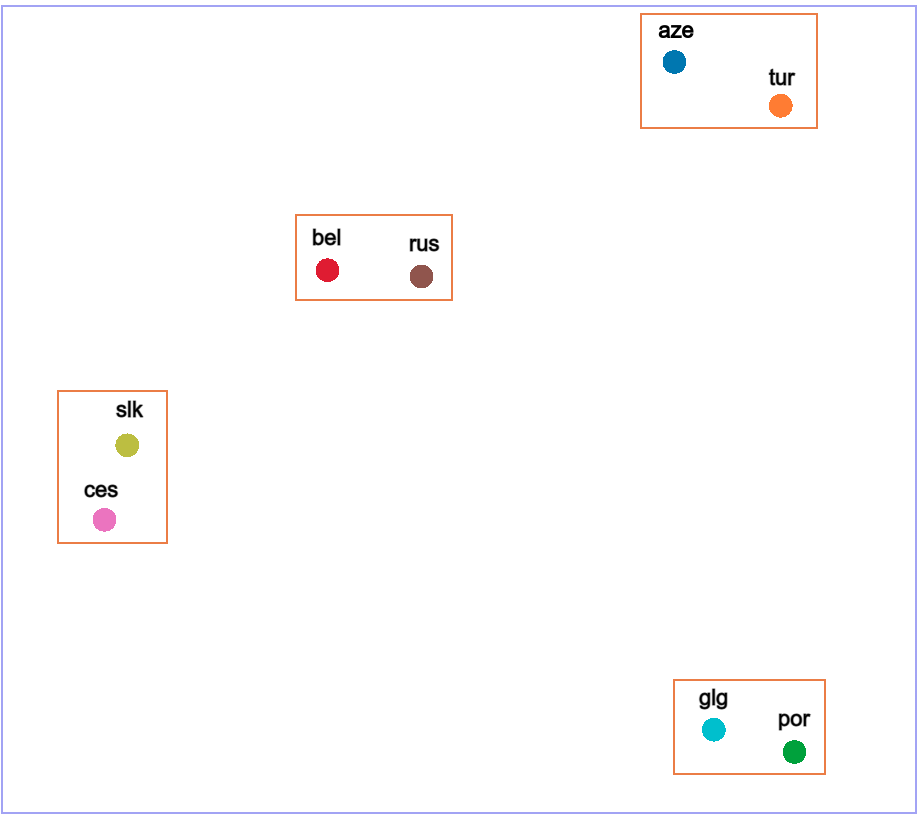
\includegraphics[width=0.9\textwidth]{ted_related}  
  \caption{TED-Related}
  \label{fig:visual-related}
\end{subfigure}
\begin{subfigure}{0.5\textwidth}
  \centering
  % include second image
  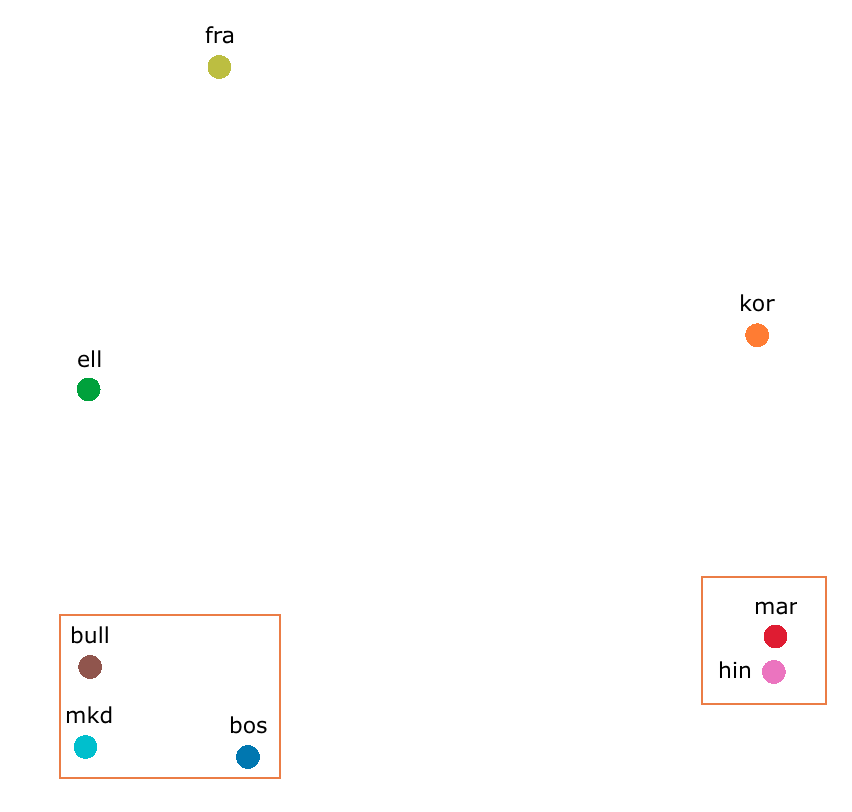
\includegraphics[width=0.85\textwidth]{ted_diverse}  
  \caption{TED-Diverse}
  \label{fig:visual-diverse}
\end{subfigure}
\caption{Visualization of languages according to their dropout masks (a large vector concatenating the dropping masks of all the layers of the model) constructed by PCA.}
\label{fig:visual}
\end{figure*}

% \begin{figure*}[h!]
% \begin{subfigure}{0.5\textwidth}
%   \centering
%   % include first image
%   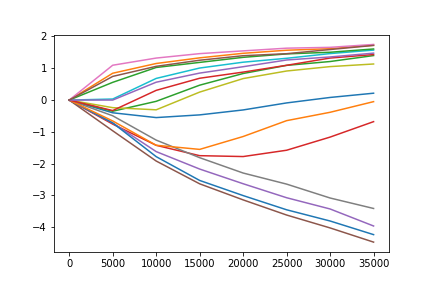
\includegraphics[width=0.9\textwidth]{phi_ted_related_o2m}  
%   \caption{TED-Related}
%   \label{fig:phi-related}
% \end{subfigure}
% \begin{subfigure}{0.5\textwidth}
%   \centering
%   % include second image
%   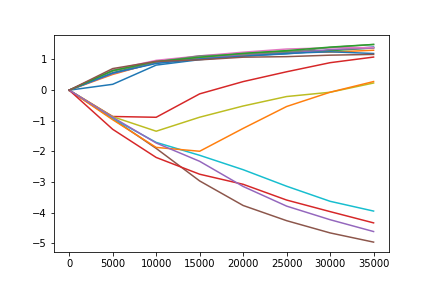
\includegraphics[width=0.85\textwidth]{phi_ted_diverse_o2m}  
%   \caption{TED-Diverse}
%   \label{fig:phi-diverse}
% \end{subfigure}
% \caption{$\Phi_L^{0}$ in O2M experiments}
% \label{fig:phi}
% \end{figure*}
\subsection{Ablation study}
We discuss here the choice of the hyper-parameters $k$, the number of activated nodes in each layer, and its impact on the sharing level between the tasks. Table~\ref{tab:K} reports the variance of performance when the number of activated nodes is changed and the sharing level between tasks decreases accordingly.
\begin{table}[h!]
  \centering
  \begin{tabular}{|c|c|c|} \hline
    $k$ & \domain{avg} & sharing rate \\ \hline 
    8 & 18.1 & 0.63\\
    10 & 19.15 & 0.73\\
    12 & 19.33 & 0.78\\
    14 & 19.44 & 0.88\\
    \hline
  \end{tabular}
  \caption{Variation of the performance w.r.t $k$, while we fix $n_p=16$ (o2m-related experiment).}
  \label{tab:K}
\end{table}
In addition, we also report in this section the effect of not choosing the number of groups $n_p$, which is assigned to 16 in the comparison of \system{LaMGD} and the contrasting methods. We show that setting $n_p$ to the layer's size, which means the group size is 1, has a very similar performance as choosing $n_p$ heuristically (Table~\ref{tab:K2}). 
\begin{table}[h!]
  \centering
  \begin{tabular}{|c|c|c|} \hline
    $k$/$n_p$ & \domain{avg} \\ \hline 
    12 / 16 & 19.33\\
    384 / 512 & 19.26\\
    \hline
  \end{tabular}
  \caption{Setting the size of group to 1 (o2m-related experiment). The quota of activated nodes is keep unchanged to $75$\%}
  \label{tab:K2}
\end{table}

\section{Related work}\label{sec:related}
Multidomain and multilingual translation systems have received considerable attention in the recent years, and a exhaustive survey is beyond the goal of this paper. Domain adaptation for neural MT is surveyed in \citep{Chu17comparison}, while multidomain MT systems are notably studied in \cite{Saunders21Asurvey,Pham21revisiting}; for multilingual MT, the reader is referred eg.\ to \citep{Chu18multilingual,dabre20survey}. We focus on the most relevant subset of this literature below.

\textbf{Language similarity} The methods developed by \citep{sen19multilingual,kong21multilingual} use language proximity to design parameter sharing strategies. The authors propose a multi-decoder model sharing the same encoder among languages and routing languages in different families to different decoders. These approaches share the same interest in expressing the proximity between tasks in the selection of task-specific parameters as our approach. However, our method learn the selection from a latent commonality in data instead of using a predefined selection such as "One language family per decoder" in \citep{kong21multilingual}.

\textbf{Language-specific sub-networks}. \done\todo{}\citet{Frankle19Lottery,liu18rethinking} study techniques to identify the most important parameters for the current task, so that masking the less important parameters during training does not hurt performance. \citet{lin21learning} adapts this idea for multilingual NMT, trying to identify language dependent subsets of parameters by pruning a fine-tuned model. Our approach also aims to map sub-networks to tasks: we do so by masking the output of each layer, rather than masking parameters. Furthermore, \citet{lin21learning} computes the masks via a heuristic selection; while our approach learns the masks with variational techniques.

\textbf{Sparse Transformer} The idea of adaptive sparsity is studied in several works. For instance, \citet{xian20deep} propose to use a variable depth for different tasks. The authors aimed to match the depth of the sub-network to the complexity of the task. \citet{Gong21pay,Gong21adaptive} also take an interest in the adaptive sparse Transformers, in which differ each task triggers the selection of specific heads in multi-head attention, layers, and blocks in feedforward matrices. Mixture-of-experts (MoE) constitute another effective approach to achieve sparsity. Using the Transformer architecture, the GShard model replaces a single feedforward (FFN) sub-layer with an MoE module consisting of multiple FFN sub-layers \citep{lepikhin21gshard,william21switch}.

\textbf{Adapter modules} Adapters have proven to be very efficient for multi-task NLP \citep{houlsby19parameter,Bapna19simple,Pham20Study,pfeiffer20adapterhub}. In a nutshell, this technique consists in plugging several so-called adapter modules to the intermediate layers of a pretrained Transformer and finetuning these adapters on the downstream tasks. Adapters can also be trained without supervision for multilingual translation \citep{Philip20monolingual}. However, the hard-coded separation between the domains of different tasks may lead to a catastrophic forgetting effect \citep{pfeiffer21adapterfusion}, which is a common problem in multi-task modeling using neural networks \citep{Michael89catastrophic}. In multidomain translation, \citet{Pham21revisiting} recently demonstrated the brittleness of adapters against fuzzy domain separations, out-of-domain distributions, and erroneous domain tags. Several subsequent studies have aimed to mitigate this weakness through a mixture of expert mechanism (e.g.\ \cite{pfeiffer21adapterfusion}).

\citet{biao21share} propose to learn to route between shared and language-specific representations with a conditional language-specific routing while training the parameters of the underlying Transformer. This method is related to the FusionAdapters of \citet{pfeiffer21adapterfusion}. Both approaches aim to select between shared and task-specific representations. The proximity between tasks is not taken into account in the routing mechanism. We propose a different approach to the problem of multi-task routing in the underlying network.

\section{Conclusions and outlook}\label{sec:conclusion}
In this work, we have presented a novel method for multdomain and multilingual translation. It allows us to jointly search for an optimal assignment of sub-networks to tasks and to learn the parameters of the underlying network. Our method relies on a sound mathematical framework and an end-to-end optimization procedure; it only adds a small number of extra parameters. The additional training cost is also reasonable, amounting to 100k iterations in the multidomain setting, given the observed gains in performance.\fyDone{There is a computational cost = 100k iterations} Experimentally, we achieve a large improvement over a Transformer baseline; our performance are also comparable to that of a strong a multi-task baseline using residual adapter modules which rely on a large number of extra parameters. For multilingual translation, our model outperforms multilingual Transformer and Language Adapters in 3 our of 4 settings. LAMGD seems specially beneficial for training languages with little parallel data, which can take advantage of the resources that are available for related languages. Besides, we provided an thorough analysis of the similarities between learned sub-networks and demonstrate a strong correlation between the learned similarities and the proximity of the corresponding tasks (domain or language).

There are several ways in which our methodology can be improved. In future work, we would first like to provide an complete variational framework to model both the number of groups, $k$ and the selection of the dropout masks. Second, we also intend to dispense with the domain information during inference: this would mean replacing the dependency on $d$ in the variational distribution by a dependency on the input $x$. Another interesting direction will be to consider adapting the size and capacity allocated to each domain / language, depending on the difficulty of the associated translation task. Addressing these questions will allow to us replace heuristic choices in the architecture design with an increased dependency on the training data.

\section{Ethical Considerations}
MT technologies are generally intended to facilitate cross-lingual as well as cross-cultural communications. The methods presented here are notably interesting in the view to improve MT from and into English for low-resource languages, subject to the availability of data for a related language. We acknowledge that (a) our results should ultimately be backed-up large scale experiments involving much more languages -- even though this goes against the idea of limiting the computing cost our experiments; (b) better architectures and training regimes can improve the translation quality for low-resource languages, yet will not solve the problem entirely. This means that additional work focusing specifically on developing resources for these languages should remain an important objective for future work.

\section{Acknowledgements}
This work was granted access to the Jean Zay HPC resources of [TGCC/CINES/IDRIS] under the allocation 2020-[AD011011270] made by GENCI (Grand Equipement National de Calcul Intensif).

\bibliography{bibliography}
\bibliographystyle{acl_natbib}
\appendix
\section{Appendix A}
\label{appendix:a}
This section explains how to compute $\hat{m}_l^d(\tau)$ by solving the optimization problem \eqref{eq:soft-top-k} and then how to compute the gradients $\frac{\partial \hat{m}_l^d(\tau)}{\partial \Phi_l^d}$.

First, to solve \eqref{eq:soft-top-k} we follow the same approach as in \cite{amos19lml,amos20differential} by applying the Karush–Kuhn–Tucker (KKT) conditions to~\eqref{eq:soft-top-k}. The solution of \eqref{eq:soft-top-k} will have the following form:
\begin{align}
\hat{m}_l^d(\tau) &= \sigma(\frac{g_l^d + \Phi_l^d + \bar{\nu}}{\tau}) \label{eq:soft-m}
\end{align}
in which $\sigma(.)$ is the sigmoid function and $\bar{\nu}$ is the solution of the following equation:
\begin{align}
\displaystyle{\mathop{\sum}_{i=1}^{n_p}} \sigma(\frac{g_l^d(i) + \Phi_l^d(i) + \nu}{\tau}) = k \label{eq:nu}
\end{align}

Because sigmoid is monotonically increasing, equation~\eqref{eq:nu} has a unique solution. Furthermore,  because of the smoothness of $g(\nu,\Phi_l^d) = \displaystyle{\mathop{\sum}_{i=1}^{n_p}} \sigma(\frac{g_l^d(i) + \Phi_l^d(i) + \nu}{\tau})$ w.r.t $\nu$ and $\Phi_l^d$, we can perform the implicit differentiation of its solution $\bar{\nu}$ w.r.t $\Phi_l^d$ as below, even though the solution of \eqref{eq:nu} does not have an explicit form.

\begin{align*}
  &\frac{\partial g}{\partial \bar{\nu}} \times \frac{\partial \bar{\nu}}{\partial \Phi_l^d} + \frac{\partial g}{\partial \Phi_l^d} = 0 \\
& \Rightarrow \frac{\partial \bar{\nu}}{\partial \Phi_l^d} = - \big(\frac{\partial g}{\partial \bar{\nu}}\big)^{-1} \times \frac{\partial g}{\partial \Phi_l^d}
\end{align*}

Because the differentiation of sigmoid has exact forms, $\frac{\partial g}{\partial \nu}$ and $\frac{\partial g}{\partial \Phi_l^d}$ also have exact form. Therefore, we do not need autograd to compute the implicit gradient $\frac{\partial \nu}{\partial \Phi_l^d}$. The gradient of $\hat{m}_l^d(\tau)$ w.r.t $\Phi_l^d$ is computed as follows:
\begin{align}
\hspace{-3.em}
  \frac{\partial \hat{m}_l^d(\tau)}{\partial \Phi_l^d} = & \frac{\partial \hat{m}_l^d(\tau)}{\partial \nu} \times \frac{\partial \nu}{\partial \Phi_l^d} +  \nonumber \\
  & \quad \frac{1}{\tau} \frac{exp(\frac{g_l^d(i) + \Phi_l^d(i) + \nu}{\tau})}{(1+exp(\frac{g_l^d(i) + \Phi_l^d(i) + \nu}{\tau}))^2}
\end{align}

In our algorithm, we solve \eqref{eq:nu} by binary search. The convergence of binary search is extremely fast and assured by the monotonicity of $g(\nu,\Phi_l^d)$. In our experiments, we set the search range to $[-100,100]$.

Finally, we need to prove that $\lim_{\tau \rightarrow 0}\hat{m}_l^d(\tau) = \tilde{m}_l^d$. We assume $g_l^d(i_1) + \Phi_l^d(i_1) > g_l^d(i_2) + \Phi_l^d(i_2) > \cdots > g_l^d(i_{n_p}) + \Phi_l^d(i_{n_p})$.

Because:
\begin{align*}
\lim_{\tau \rightarrow 0} \sigma(\frac{g_l^d(i) + \Phi_l^d(i) + \nu}{\tau}) = \\
= \begin{cases}
      1, & \text{if}\ \tau > - (g_l^d(i) + \Phi_l^d(i)), \\
      0, & \text{if}\ \tau < - (g_l^d(i) + \Phi_l^d(i)), \\
      \frac{1}{2} &\text{otherwise}\\
    \end{cases}
%% \hspace{-3.em}
%  \lim_{\tau \rightarrow 0} \sigma(\frac{g_l^d(i) + \Phi_l^d(i) + \nu}{\tau}) & = \\
%  \quad \begin{cases}
%    1, & \text{if}\ \tau > - (g_l^d(i) + \Phi_l^d(i)), \\
%    0, & \text{if}\ \tau < - (g_l^d(i) + \Phi_l^d(i)), \\
%    \frac{1}{2} &\text{otherwise}\\
%  \end{cases}
\end{align*}

and 

\begin{align*}
\displaystyle{\mathop{\sum}_{i=1}^{n_p}} \sigma(\frac{g_l^d(i) + \Phi_l^d(i) + \nu}{\tau}) = k
\end{align*}
there exist $\epsilon$ such that $\forall \tau < \epsilon$, the solution $\bar{\nu}$ of \eqref{eq:nu} satisfies $- (g_l^d(i_{k+1}) + \Phi_l^d(i_{k+1})) > \bar{\nu} > - (g_l^d(i_k) + \Phi_l^d(i_k))$. Furthermore, because sigmoid is monotonically increasing,

\begin{align*}
&\sigma(\frac{g_l^d(i) + \Phi_l^d(i) - (g_l^d(i_{k}) + \Phi_l^d(i_{k}))}{\tau}) < \hat{m}_l^d(\tau)(i)  \\
& < \sigma(\frac{g_l^d(i) + \Phi_l^d(i) - (g_l^d(i_{k+1}) + \Phi_l^d(i_{k+1}))}{\tau}) 
\end{align*}

By taking the limit on both sides, we get the following results:
\begin{align*}
\lim_{\tau \rightarrow 0} \hat{m}_l^d(\tau)(i_u) = \begin{cases}
      1, & \text{if}\ u > k \\
      0, & \text{if}\ u < k \\
    \end{cases}
\end{align*}

And, because $ \displaystyle{\mathop{\sum}_{u=1}^{n_p}}\hat{m}_l^d(\tau)(i_u) = k$, by taking the limit on both sides, we will have $\lim_{\tau \rightarrow 0} \hat{m}_l^d(\tau)(i_k) = 1$. Finally, we have

\begin{align*}
\lim_{\tau \rightarrow 0} \hat{m}_l^d(\tau)(i_u) = \begin{cases}
      1, & \text{if}\ u \geqslant k \\
      0, & \text{if}\ u < k \\
    \end{cases}
\end{align*}

which is equivalent to $\lim_{\tau \rightarrow 0}\hat{m}_l^d(\tau) = \tilde{m}_l^d$.

\section{Appendix B}
\label{appendix:b}
In this section, we give a simple proof of inequality~\eqref{eq:entropy}. In fact, we only need to prove $\mathbb{H} \big[ P(i_1,\cdots,i_k | \Phi_l^d) \big] \geqslant \mathbb{H} \big[ P(i_1 | \Phi_l^d) \big]$. The proof is as follows:
\begin{align*}
&\mathbb{H} \big[ P(i_1\cdots i_k | \Phi_l^d) \big] = - \displaystyle{\mathop{\mathbb{E}}_{i_1\cdots i_k | \Phi_l^d}} \big[ \text{log}P(i_1 \cdots i_k | \Phi_l^d) \big] \\
&= -\!\! \!\!\!\! \displaystyle{\mathop{\mathbb{E}}_{i_1\cdots i_k | \Phi_l^d}} \big[ \displaystyle{\sum_{j=2}^k}\text{log}P(i_j | i_1 \cdots j_{j-1},\Phi_l^d) +  \text{log} P(i_1 | \Phi_l^d) \big] \\
&\geqslant -\!\! \!\! \!\!\displaystyle{\mathop{\mathbb{E}}_{i_1 \cdots i_k | \Phi_l^d}} \big[ \text{log} P(i_1 | \Phi_l^d) \big] \\
&= -\displaystyle{\mathop{\mathbb{E}}_{i_1 | \Phi_l^d}} \big[ \text{log} P(i_1 | \Phi_l^d) \big] = \mathbb{H} \big[ P(i_1 | \Phi_l^d) \big]
\end{align*}
\section{Appendix C}
\begin{figure}[H]
\centering{
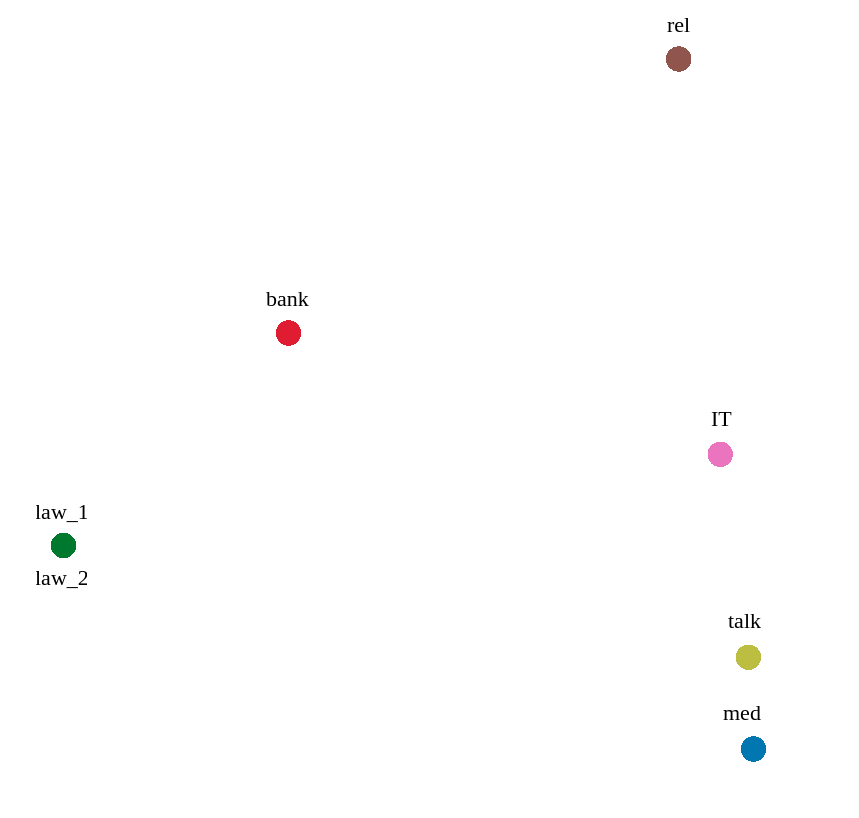
\includegraphics[width=0.5\textwidth,frame]{multi_domain}}
\caption{Visualization of domains according to their dropout masks (a large vector concatenating the dropping masks of all the layers of the model) constructed by PCA.}
\label{fig:domain}
\end{figure}
\section{Appendix D}
\begin{breakablealgorithm}
\caption{Training \system{LaMGD}} \label{alg:mdmt}
\begin{algorithmic}[1]
  \REQUIRE {%    
  \begin{itemize}
    \setlength{\itemsep}{-1pt}    \setlength{\parsep}{0pt}
  \item[] 
  \item $n_d$ corpora $C^d, d \in [1, \dots,n_d]$ for $n_d$ domains equiped by an empirical distribution $D_d(x)$
  \item number of groups: $n_p$; number of retained groups: $k$ 
  \item $i=0$; $iter\_num$
 \end{itemize}}
\REPEAT 
\STATE{Pick a batch from domain $d$}
\STATE{Sample $\forall l, \forall p:  g_l^d(p) \displaystyle{\mathop{\sim}^{\text{i.i.d}}} \operatorname{Gumbel}(0,1)$}
\STATE{Solve the equation $\forall l$
\begin{align*}
\displaystyle{\mathop{\sum}_{i=1}^{n_p}} \sigma(\frac{g_l^d(i) + \Phi_l^d(i) + \nu}{\tau}) = k
\end{align*}
using binary search}
\STATE{Compute mask of each layer:
\begin{align*}
\forall l, \hat{m}_l^d(\tau) &= \sigma(\frac{g_l^d + \Phi_l^d + \bar{\nu}}{\tau})
\end{align*}}
\STATE{Apply masks to their corresponding layer:
\begin{align*}
  \forall l \in [0,\cdots, L-1]: \tilde{h}^l &= h^l \odot r_l^d ,\\
  h^{l+1} &= \operatorname{LAYER}^{l+1}(\tilde{h}^l) ,
\end{align*}
}
\STATE{Compute gradient of training loss over the underlying Transformer:
$$\Delta_{\theta} = \frac{\partial L}{\partial \theta}$$}
\STATE{Compute gradient over the $\operatorname{Soft-Top-K}$ masks:
$$\frac{\partial D}{\partial \hat{m}_l^d(\tau)}$$}
\STATE{Compute implicit gradient of the $\operatorname{Soft-Top-K}$ masks over $\Phi_l^d$:
$$\frac{\partial \bar{\nu}}{\partial \Phi_l^d} = - \big(\frac{\partial g}{\partial \bar{\nu}}\big)^{-1} \times \frac{\partial g}{\partial \Phi_l^d}$$
$$\frac{\partial \hat{m}_l^d(\tau)}{\partial \Phi_l^d} = \frac{\partial \hat{m}_l^d(\tau)}{\partial \nu} \times \frac{\partial \nu}{\partial \Phi_l^d}  + $$
$$ \quad\quad \frac{1}{\tau} \frac{exp(\frac{g_l^d(i) + \Phi_l^d(i) + \nu}{\tau})}{(1+exp(\frac{g_l^d(i) + \Phi_l^d(i) + \nu}{\tau}))^2}$$}
\STATE{Compute the gradient the training over $\Phi_l^d$:
$$ \Delta_{\Phi_l^d} = \frac{\partial D}{\partial \hat{m}_l^d(\tau)}  \frac{\partial \hat{m}_l^d(\tau)}{\partial \Phi_l^d} + \frac{\partial \mathbb{H} \big[ \operatorname{softmax}(\Phi_l^d)\big] }{\partial \Phi_l^d} $$}
\STATE{Update $\theta$ and $\Phi_l^d$ with their gradients}
\STATE{$i=i+1$}
\UNTIL{$i> iter\_num$}
\end{algorithmic}
\end{breakablealgorithm}

\end{document}

































%\en